\documentclass{beamer}

\mode<presentation>
{
  \usetheme{Madrid}      % or try Darmstadt, Madrid, Warsaw, ...
  \setbeamertemplate{navigation symbols}{}
  \setbeamertemplate{caption}[numbered]
} 

\colorlet{beamer@blendedblue}{black}

\usepackage[french]{babel}
\usepackage[utf8]{inputenc}
\usepackage[T1]{fontenc}
%\usepackage[squaren,cdot]{SIunits}
\usepackage{graphicx}
\usepackage{listings}
\usepackage{wrapfig}

\graphicspath{}

\logo{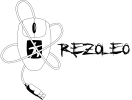
\includegraphics[height=0.8cm]{../../rezoleo.png}\vspace{10pt}\hspace{20pt}}
\title{Introduction aux réseaux}
\author{LEDER "Ziman" Simon}
\institute{Rezoleo\\}
\date{\today}

\begin{document}
	
	\maketitle

	\begin{frame}
		\frametitle{Sommaire} 
		\tableofcontents
	\end{frame}

\section{Topologie}
	\begin{frame}{Topologie}{Topologie en bus}
		\begin{center}
			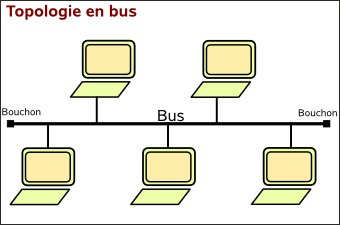
\includegraphics[scale = 0.5]{Bus.jpg}\\
		\end{center}
		La Topologie en Bus : On dit qu’un réseau a une topologie en bus quand toutes les stations sont reliées à un câble unique.
	\end{frame}

	\begin{frame}{Topologie en anneau}
		\begin{center}
			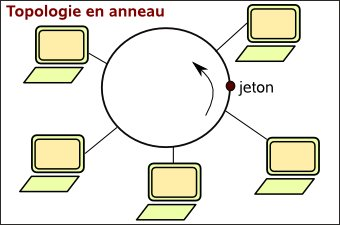
\includegraphics[scale = 0.5]{Anneau.jpg}\\
		\end{center}
			La Topologie en Boucle (Anneau) : Un réseau a une topologie en anneau quand toutes ses stations sont connectées en chaîne les unes aux autres par une liaison bipoint et la dernière à la
	\end{frame}

	\begin{frame}{Topologie en étoile}
		\begin{center}
			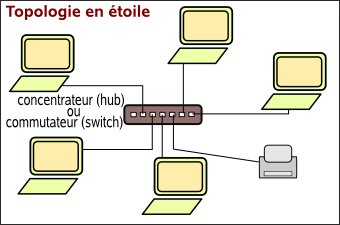
\includegraphics[scale = 0.6]{Etoile.jpg}
		\end{center}
		La Topologie en Étoile : Un réseau à une topologie en étoile quand les stations sont raccordées par des liaisons point-à-point à des noeuds qui sont chargés de ré-émettre les trames.
	\end{frame}

	\begin{frame}{Topologie en arbre}
		\begin{center}
			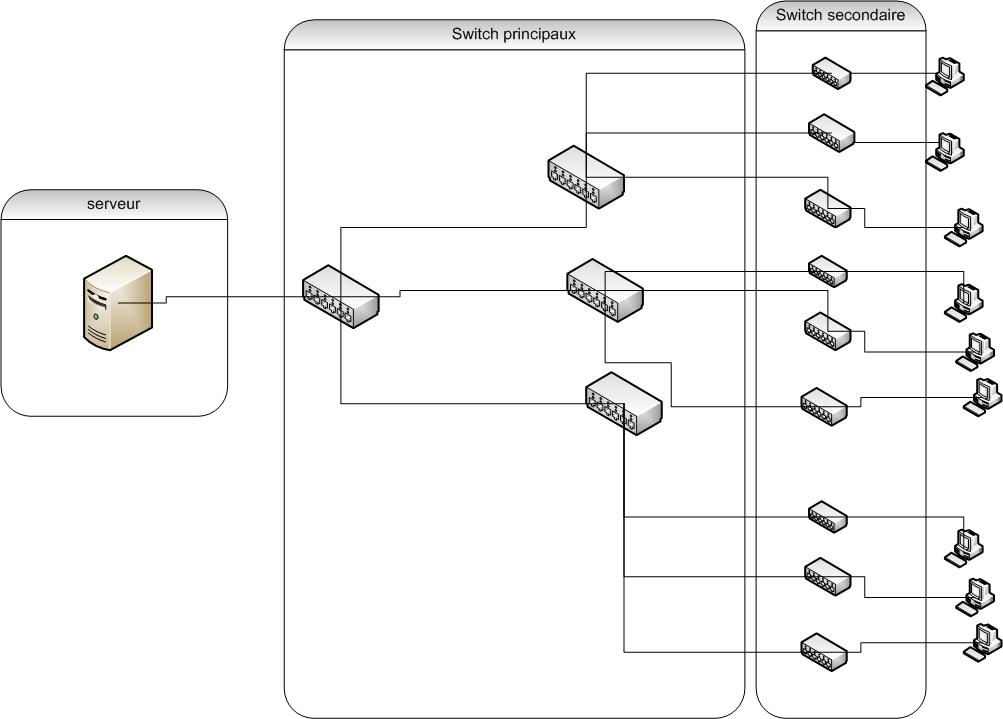
\includegraphics[scale = 0.3]{Arbre.jpg}
		\end{center}
			La Topologie en Étoile : Un réseau à une topologie en étoile quand les stations sont raccordées par des liaisons point-à-point à des noeuds qui sont chargés de ré-émettre les trames.
	\end{frame}

	\begin{frame}{Topologie en maille}
		\begin{center}
			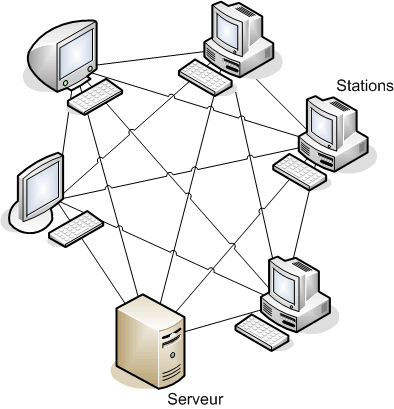
\includegraphics[scale = 0.4]{Maille.png}
		\end{center}
			La Topologie en Étoile : Un réseau à une topologie en étoile quand les stations sont raccordées par des liaisons point-à-point à des noeuds qui sont chargés de ré-émettre les trames.
	\end{frame}

\section{Le modèle OSI}

	\begin{frame}{Le modèle OSI}
		Le modèle OSI (de l'anglais Open Systems Interconnection, « Interconnexion de systèmes ouverts ») d'interconnexion en réseau des systèmes ouverts est un modèle de communications entre ordinateurs proposé par l'ISO (Organisation internationale de normalisation). Il décrit les fonctionnalités nécessaires à la communication et l'organisation de ces fonctions.
	
	\end{frame}

	\begin{frame}{le modèle OSI}
		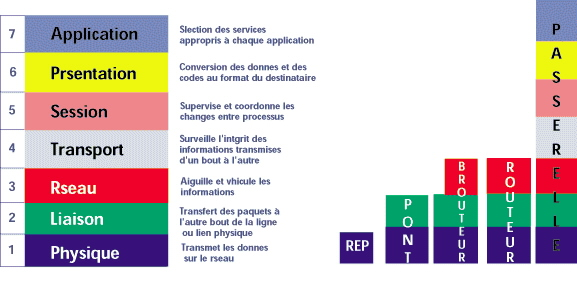
\includegraphics[scale = 0.8]{OSI.jpg}\\
	\end{frame}

	\begin{frame}{encapsulation}
		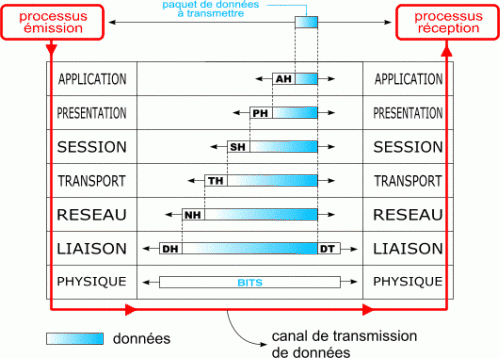
\includegraphics[scale = 0.65]{Encaps.png}\\
	\end{frame}

\section{Le modèle TCP/IP}

	\begin{frame}
		\begin{center}
			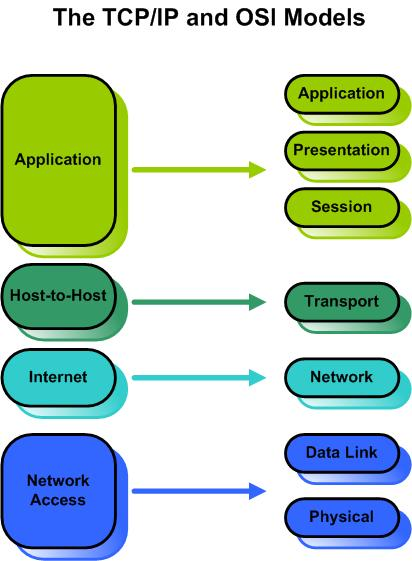
\includegraphics[scale = 0.55]{TCPIP.png}\\
		\end{center}
	\end{frame}

\end{document}